% The document class supplies options to control rendering of some standard
% features in the result.  The goal is for uniform style, so some attention 
% to detail is *vital* with all fields.  Each field (i.e., text inside the
% curly braces below, so the MEng text inside {MEng} for instance) should 
% take into account the following:
%
% - author name       should be formatted as "FirstName LastName"
%   (not "Initial LastName" for example),
% - supervisor name   should be formatted as "Title FirstName LastName"
%   (where Title is "Dr." or "Prof." for example),
% - degree programme  should be "BSc", "MEng", "MSci", "MSc" or "PhD",
% - dissertation title should be correctly capitalised (plus you can have
%   an optional sub-title if appropriate, or leave this field blank),
% - dissertation type should be formatted as one of the following:
%   * for the MEng degree programme either "enterprise" or "research" to
%     reflect the stream,
%   * for the MSc  degree programme "$X/Y/Z$" for a project deemed to be
%     X%, Y% and Z% of type I, II and III.
% - year              should be formatted as a 4-digit year of submission
%   (so 2014 rather than the academic year, say 2013/14 say).

\documentclass[ oneside,tikz,% the name of the author
                    author={Joshua Felmeden},
                % the degree programme: BSc, MEng, MSci or MSc.
                    degree={MEng},
                % the dissertation    title (which cannot be blank)
                     title={Semantic Analysis of Financial Headlines Based on Realised Stock Returns},
                % the dissertation subtitle (which can    be blank)
                  subtitle={Research}]{dissertation}

\usepackage{tabularx}
\usepackage{booktabs}
\usepackage{multirow}
\usepackage{pgfplots}
\usepackage{pgfplotstable}
\usepackage{siunitx}
\usepackage{graphicx}
\pgfplotsset{compat=1.12}
\usetikzlibrary{
    pgfplots.dateplot,
}
\usepackage{subcaption}
\newcommand\setrow[1]{\gdef\rowmac{#1}#1\ignorespaces}
\newcommand\clearrow{\global\let\rowmac\relax}
\clearrow

\begin{document}

% =============================================================================

% This section simply introduces the structural guidelines.  It can clearly
% be deleted (or commented out) if you use the file as a template for your
% own dissertation: everything following it is in the correct order to use 
% as is.

% \section*{Prelude}
% \thispagestyle{empty}

% A typical dissertation will be structured according to (somewhat) standard 
% sections, described in what follows.  However, it is hard and perhaps even 
% counter-productive to generalise: the goal is {\em not} to be prescriptive, 
% but simply to act as a guideline.  In particular, each page count given is
% important but {\em not} absolute: their aim is simply to highlight that a 
% clear, concise description is better than a rambling alternative that makes
% it hard to separate important content and facts from trivia.

% % You can use this document as a \LaTeX-based~\cite{latexbook1,latexbook2} 
% template for your own dissertation by simply deleting extraneous sections
% and content; keep in mind that the associated {\tt Makefile} could be of
% use. %, in particular because it automatically executes \mbox{\BibTeX} to 
% deal with the associated bibliography. 
% Alternatively, upload this template, dissertation.bib, dissertation.cls, 
% dtklogos.sty and the "logo" folder to Overleaf (an online \LaTeX editor and compiler) and work on your thesis there.

% \textbf{Do not include this section in your final dissertation --- just delete it from the source.}

% =============================================================================

% This macro creates the standard UoB title page by using information drawn
% from the document class (meaning it is vital you select the correct degree 
% title and so on).

\maketitle

% After the title page (which is a special case in that it is not numbered)
% comes the front matter or preliminaries; this macro signals the start of
% such content, meaning the pages are numbered with Roman numerals.

\frontmatter


%\lstlistoflistings

% The following sections are part of the front matter, but are not generated
% automatically by LaTeX; the use of \chapter* means they are not numbered.

% -----------------------------------------------------------------------------

\chapter*{Abstract}

{\bf A compulsory section, of at most 300 words} 
\vspace{1cm} 

\noindent
This section should pr\'{e}cis the project context, aims and objectives,
and main contributions (e.g., deliverables) and achievements; the same 
section may be called an abstract elsewhere.  The goal is to ensure the 
reader is clear about what the topic is, what you have done within this 
topic, {\em and} what your view of the outcome is.

The former aspects should be guided by your specification: essentially 
this section is a (very) short version of what is typically the first 
chapter. If your project is experimental in nature, this should include 
a clear research hypothesis.  This will obviously differ significantly
for each project, but an example might be as follows:

\begin{quote}
My research hypothesis is that a suitable genetic algorithm will yield
more accurate results (when applied to the standard ACME data set) than 
the algorithm proposed by Jones and Smith, while also executing in less
time.
\end{quote}

\noindent
The latter aspects should (ideally) be presented as a concise, factual 
bullet point list.  Again the points will differ for each project, but 
an might be as follows:

\begin{quote}
\noindent
\begin{itemize}
\item I spent $120$ hours collecting material on and learning about the 
      Java garbage-collection sub-system. 
\item I wrote a total of $5000$ lines of source code, comprising a Linux 
      device driver for a robot (in C) and a GUI (in Java) that is 
      used to control it.
\item I designed a new algorithm for computing the non-linear mapping 
      from A-space to B-space using a genetic algorithm, see page $17$.
\item I implemented a version of the algorithm proposed by Jones and 
      Smith in [6], see page $12$, corrected a mistake in it, and 
      compared the results with several alternatives.
\end{itemize}
\end{quote}

% -----------------------------------------------------------------------------


\chapter*{Dedication and Acknowledgements}

% {\bf A compulsory section}
% \vspace{1cm} 

% \noindent
% It is common practice (although totally optional) to acknowledge any
% third-party advice, contribution or influence you have found useful
% during your work.   include support from friends or family, 
% the input of your Supervisor and/or Advisor, external organisations 
% or persons who  have supplied resources of some kind (e.g., funding, 
% advice or time), and so on.

I am very fortunate to work with my superviser Rami Chehab, who assisted in my research greatly and inspired the vast quantity of this project. He has been a great mentor.

I would also like to thank my friends and family for always being there for me, especially when the going gets rough. You guys really helped make this university experience what it was.


% -----------------------------------------------------------------------------


% \chapter*{COVID-19 Statement}

% {\bf An optional section, of at most 800 words} 
% \vspace{1cm} 

% \noindent
% A summary of any planned research activities disrupted by Covid-19 restrictions and the extent to which it was possible to adapt the work in those changed circumstances. If the project was able to go forward as planned, you can safely remove this section without losing any marks. The following may be included:

% \begin{itemize}
% \item Details of any planned research activities curtailed by the pandemic because of, for example, lack of access to facilities, libraries, archives, research participants, fieldwork, etc. Information on any curtailed training should be included only insofar as it relates to the impact on research activities and on the dissertation.

% \item An acknowledgement of the anticipated contribution and value to the dissertation if those research activities had not been curtailed and what was possible to include in the dissertation in the circumstances, including where alternative choices were made to adapt the work and whether there are any weaknesses that could not be overcome.

% \item Any other relevant factors on the impact of Covid-19 on research activities and on the contents of the dissertation.

% \item Details of any research activities required by the examiners as part of a resubmission that were curtailed by the pandemic may be included in a new or revised Covid-19 statement in the resubmitted dissertation.
% \end{itemize}

% -----------------------------------------------------------------------------

% This macro creates the standard UoB declaration; on the printed hard-copy,
% this must be physically signed by the author in the space indicated.

\makedecl



% -----------------------------------------------------------------------------

% LaTeX automatically generates a table of contents, plus associated lists 
% of figures and tables.  These are all compulsory parts of the dissertation.

\tableofcontents
\listoffigures
\listoftables

% -----------------------------------------------------------------------------



\chapter*{Ethics Statement}

{\bf A compulsory section} 
\vspace{1cm} 

In almost every project, this will be one of the following statements:
    \begin{itemize}
        \item ``This project did not require ethical review, as determined by my supervisor, [fill in name]''; or
        \item ``This project fits within the scope of ethics application 0026, as reviewed by my supervisor, [fill in name]''; or
        \item ``An ethics application for this project was reviewed and approved by the faculty research ethics committee as application [fill in number]''.
    \end{itemize}
    
See Section 3.2 of the unit Handbook for more information. If something went wrong and none of those three statements apply, then you should instead explain what happened.


% -----------------------------------------------------------------------------

% \chapter*{Summary of Changes}

% {\bf A conditional section} 
% \vspace{1cm} 

% If and only if the dissertation represents a resubmission (e.g., as the result of
% a resit), this section is compulsory: the content should summarise all
% non-trivial changes made to the initial submission.  Otherwise you can
% omit it, since a summary of this type is clearly nonsensical.

% When included, the section will ideally be used to highlight additional
% work completed, and address criticism raised in any associated feedback.
% Clearly it is difficult to give generic advice about how to do so, but
% an example might be as follows:

% \begin{quote}
% \noindent
% \begin{itemize}
% \item Feedback from the initial submission criticised the design and 
%       implementation of my genetic algorithm, stating ``there seems 
%       to have been no attention to computational complexity during the
%       design, and obvious methods of optimisation are missing within
%       the resulting implementation''.  Chapter $3$ now includes a
%       comprehensive analysis of the algorithm, in terms of both time
%       and space.  While I have not altered the algorithm itself, I
%       have included a cache mechanism (also detailed in Chapter $3$)
%       that provides a significant improvement in average run-time.
% \item I added a feature in my implementation to allow automatic rather
%       than manual selection of various parameters; the experimental
%       results in Chapter $4$ have been updated to reflect this.
% \item Questions after the presentation highlighted a range of related
%       work that I had not considered: I have make a number of updates 
%       to Chapter $2$, resolving this issue.
% \end{itemize}
% \end{quote}

% -----------------------------------------------------------------------------

\chapter*{Supporting Technologies}

% {\bf An optional section}
% \vspace{1cm} 

% \noindent
% This section should present a detailed summary, in bullet point form, 
% of any third-party resources (e.g., hardware and software components) 
% used during the project.  Use of such resources is always perfectly 
% acceptable: the goal of this section is simply to be clear about how
% and where they are used, so that a clear assessment of your work can
% result.  The content can focus on the project topic itself (rather,
% for example, than including ``I used \mbox{\LaTeX} to prepare my 
% dissertation''); an example is as follows:

% \begin{quote}
% \noindent
% \begin{itemize}
% \item I used the Java {\tt BigInteger} class to support my implementation 
%       of RSA.
% \item I used a parts of the OpenCV computer vision library to capture 
%       images from a camera, and for various standard operations (e.g., 
%       threshold, edge detection).
% \item I used an FPGA device supplied by the Department, and altered it 
%       to support an open-source UART core obtained from 
%       \url{http://opencores.org/}.
% \item The web-interface component of my system was implemented by 
%       extending the open-source WordPress software available from
%       \url{http://wordpress.org/}.
% \end{itemize}
% \end{quote}

\begin{itemize}
      \item I used a sample of headlines from Kaggle as training and validation data (\url{https://www.kaggle.com/datasets/miguelaenlle/massive-stock-news-analysis-db-for-nlpbacktests})
      \item I used the Natural Language Toolkit to assist the preprocessing of data, using their English words and stop words data (\url{https://www.nltk.org/})
\end{itemize}


% -----------------------------------------------------------------------------

\chapter*{Notation and Acronyms}

\begin{quote}
\noindent
\begin{tabular}{lcl}
NLP               &:    &     Natural Language Processing \\
SESTM             &:    &     Semantic Extraction via Screening and Topic Modelling \\
\\
\textbf{SESTM Specific Notation} \\
$m$               &:    &     Number of words in sample \\
$n$               &:    &     Number of articles in sample \\
$d_{i,j}$         &:    &     Number of times word $j$ appears in text $i$ \\
$d_{[S],i}$       &:    &     Subset of columns where the only indices are those with sentiment \\
$D = [d_1, \dots, d_n]$ &:    & $m \times n$ Document term matrix \\
$sgn(y)$          &:    &     Sign of returns of article y \\
$\hat x$          &:    &    Expected value of variable $x$ \\
\end{tabular}
\end{quote}


% =============================================================================

% After the front matter comes a number of chapters; under each chapter,
% sections, subsections and even subsubsections are permissible.  The
% pages in this part are numbered with Arabic numerals.  Note that:
%
% - A reference point can be marked using \label{XXX}, and then later
%   referred to via \ref{XXX}; for example Chapter\ref{chap:context}.
% - The chapters are presented here in one file; this can become hard
%   to manage.  An alternative is to save the content in seprate files
%   the use \input{XXX} to import it, which acts like the #include
%   directive in C.

\mainmatter


\chapter{Introduction}
\label{chap:context}
Financial news is a widely available resource from which many investors and businesses alike glean information. It is an insight into how many different businesses function and the health of markets. If properly used, can be taken as a measure of ... Analysing the sentiment of an article has been used for a significant amount of time and is utilised for a myriad of purposes, including forecasting financial stocks.

An article is naturally formed of two parts, the headline and the article body. The bulk of the information conveyed by a given article is in the body, however, since headlines are often a summarisation of the body, it has been proven that data mining from the headline itself can be at least as useful as mining the body \{citation needed\}. The average word counts of a headline are very low, however, the vocabulary is often much higher impact on average, as this is what initially grabs the attention of a reader.

\section{What to do}

\noindent
This chapter should introduce the project context and motivate each of the proposed aims and objectives.  Ideally, it is written at a fairly high-level, and easily understood by a reader who is technically competent but not an expert in the topic itself.

In short, the goal is to answer three questions for the reader.  First, what is the project topic, or problem being investigated?  Second, why is the topic important, or rather why should the reader care about it?  For example, why there is a need for this project (e.g., lack of similar software or deficiency in existing software), who will benefit from the project and in what way (e.g., end-users, or software developers) what work does the project build on and why is the selected approach either important and/or interesting (e.g., fills a gap in literature, applies results from another field to a new problem).  Finally, what are the central challenges involved and why are they significant? 
 
The chapter should conclude with a concise bullet point list that summarises the aims and objectives.  For example:

\begin{quote}
\noindent
The high-level objective of this project is to reduce the performance 
gap between hardware and software implementations of modular arithmetic.  
More specifically, the concrete aims are:

\begin{enumerate}
\item Research and survey literature on public-key cryptography and
      identify the state of the art in exponentiation algorithms.
\item Improve the state of the art algorithm so that it can be used
      in an effective and flexible way on constrained devices.
\item Implement a framework for describing exponentiation algorithms
      and populate it with suitable examples from the literature on 
      an ARM7 platform.
\item Use the framework to perform a study of algorithm performance
      in terms of time and space, and show the proposed improvements
      are worthwhile.
\end{enumerate}
\end{quote}

% -----------------------------------------------------------------------------

\chapter{Background}
\label{chap:technical}

We begin by discussing the technical background that relate to the work in the thesis. This project evaluates and analyses the success of semantic analysis when applied to financial headlines; making use of realised stock returns as a teaching signal.

\section{Semantic Analysis}
Semantic analysis (also known as opinion mining) is the task of identifying opinions or sentiment of authors from an input of text. The ramifications of being able to programmatically extract the intended meaning of an input is extremely powerful in a variety of fields and is particularly prudent in a financial context. The nuances of natural language can sometimes make this difficult to extract, and therefore significant research has been conducted on the topic over the course of the last decades.

\subsection{Lexicon Based Methods}
The fundamental concept revolves around investigating a piece of text, and deciding on a binary classification: positive or negative. The simplest method compiles a list words with weights. Each weight corresponds to the positivity of the word (for example `great' would have a high positivity, while `terrible' would have very low). The overall sentiment of a piece of text could then be estimated by summing the individual sentiment scores of each word. The dictionary is not limited to single words, and can be expanded to include $n$-grams (phrases of $n$ words), as the context in which a word is used can dramatically change the sentiment. This may increase the accuracy of the dictionary at the cost of increased dimensionality. The dictionary itself must be compiled before it is possible to utilise this method. One of the most widely used for English text is the Harvard-IV-4 TagNeg (H4N) lexicon which is a general usage model that can be used to estimate the sentiment of a piece of text.

There are many difficulties faced with creating a dictionary of this sort, as language is often a subjective entity, leading to conflicting opinions in assigning tone to a specific word. Furthermore, the context within which a word is used can drastically change the intended sentiment of a word, for example, the word `great' is naturally a very positive word, however, if used in a sarcastic manner (e.g. `It's so great that my flight is delayed!') can invert the sentiment entirely. For this reason, simply summing the sentiment of a piece of text on a word by word scale can give an incorrect estimate.

Certain words that may have no meaning at all in one context, may have significant sentiment in another, particularly in the field of finance, where jargon dominates text. Loughran and McDonald \cite{lm-dict} conducted an investigation into the use of standard lexicons for use in analysing 10-K filing reports, which are comprehensive reports filed by companies about their financial performance. They discovered that almost 75\% of negative words found in the filings based on the H4N file were not typically negative in a financial context. For example, `liability' is a negatively charged word in a standard context, while it carries no tone at all in the context of the filings. Loughran and McDonald created their own dictionary based on these results called the Loughran McDonald dictionary that is created for the purpose of classifying 10-k filings. For these reasons, lexicon based methods work far better if the it is bespoke for the topic at hand, needing a specific dictionary for each task. 

\subsection{Usage}
Usage of these lexicons can vary greatly, with some simply summing the count of positive words and subtracting the count of negative words to end up with a simple overall word count. However, this is a very trivialised method of use and can be expanded to be far more constructive. Loughran and McDonald themselves suggest using Term Frequency Inverse Document Frequency (TF-IDF) as a method to weight the word counts alone. TF-IDF is one of the most popular term weighting schemes, and it therefore makes sense to augment these strategies with this weighting.

TF-IDF has two distinct parts, term frequency and inverse document frequency. Term frequency (TF) is the relative frequency of a term $t$ in a document $d$:
\begin{equation}
tf(t,d) =  \frac{f_{t,d}}{\sum_{t'\in d, t' \neq t} f_{t',d}}
\end{equation}

\noindent
where $f_{t,d}$ is the raw count of term $t$ in document $d$. This is one method of calculating the term frequency, however there are many variations, such as logarithmically scaled frequency ($\log(1 + f_{t,d})$), boolean frequency (1 if $t$ appears in $d$ at all, and 0 otherwise), etc.

Inverse document frequency measures how much information a word carries by its rarity. The generic equation is as follows:
\begin{equation}
idf(t,D) = \log \frac{N}{|\{d \in D: t \in d\}|}
\end{equation}

\noindent
where $N = |D|$ and $D = [d_1, d_2, \dots, d_n]$. 

Using these two components in conjuction, the final TF-IDF of a term is:
\begin{equation}
tfidf(t,d,D) = tf(t,d) \times idf(t,D)
\end{equation}

\section{Semantic Extraction via Screening and Topic Modelling}
Semantic Extraction via Screening and topic model (SESTM) is a novel text mining algorithm that makes us of a teaching signal developed by Ke et Al. in 2019 \cite{sestm}. It makes use of stock returns as a teaching signal to develop a model of sentiment words in maximally positive or negative arguments in order to be able to predict the sentiment of out of sample articles.

To begin, we assume that each headline has some sentiment score $p_i \in [0,1]$, with $p_i = 1$ being a headline with maximum positive sentiment, and $p_i = 0$ maximally negative. Our problem is ot model the distribution of returns of a headline $y_i$ given the sentiment of the headline $p_i$. Thus we have assumed:
\begin{equation}
\mathbb{P}(\text{sgn}(y_i) = 1) = g(p_i) \text{, for a monotone increasing function } g(\cdot)
\end{equation}

\noindent
where sgn($x$) returns $1$ if $x > 0$ and $-1$ otherwise. This assumption simply states that the higher the sentiment score, the higher the probability the headline has of returning positive returns.

Next, we observe the distribution of word counts in an article. We assume a vocabulary has partition
\begin{equation}
\{1,2,\dots,m\} = S \cup N
\end{equation}

\noindent
where $S$ is the set of sentiment charged words and $N$ is the set of sentiment neutral words. Thus, the distribution of sentiment charged words are the vector $d_{[S],i}$, similarly for sentiment neutral words $d_{[N],i}$, although sentiment neutral words serve as useless noise and remain unmodelled.

Utilising the work of Hoffman, we adapt latent semantic analysis (LSA) which is a technique that maps high-dimensional word count vectors to a lower dimensional representation (in our case, the realised returns) \cite{lsa}. We then assume that the vector of sentiment charged word counts are generated by a mixture multinomial model of form
\begin{equation}
d_{[S],i} \sim \text{Multinomial}(s_i, p_iO_+ + (1-p_i)O_-)
\label{multinom}
\end{equation}

\noindent
where $s_i$ is the total count of sentiment charged words in headline $i$. $O_+$ is the probability distribution and simply describes expected word counts in a maximally positive headline (namely $p_i = 1$). Similarly, $O_-$ describes expected word counts in maximally negative headlines ($p_i = 0$). Fundamentally, this model is the probability of counts for each sentiment charged word in our vocabulary, with $s_i$ trials and the outcome is modelled by $p_iO_+ + (1-p_i)O_-$. 

Using these two probability distributions, we can also gain insight into vectors of tone $T$ and frequency $F$:
\begin{equation}
F = \frac{1}{2}(O_+ + O_-), \quad T= \frac{1}{2}(O_+ - O_-)
\end{equation}

\subsection{Screening for sentiment charged words}
\label{screen-sentiment}
The first step in this algorithm is to screen for sentiment words in a collection of articles, since sentiment neutral words are a nuidance and contribute to noise. This strategy isolates the sentiment charged words and uses these alone to calculate sentiment. This is achieved by using a supervised approach with the realised returns of an associated stock, since if a word appears in headlines that result in positive returns, it is reasonable to assume that the word carries positive sentiment. Some notation will be introduced here to facilitate the discussion and explanation of the algorithm.
\begin{itemize}
      \item The sample is defined as $n$ articles producing a dictionary of $m$ words.
      \item The word count of article $i$ is recorded in vector $d_i$
      \item $D = [d_1, d_2, \dots, d_n]$ is an $m \times n$ document term matrix
      \item The count of sentiment charged words in article $i$ is defined as the submatrix $d_{[S],i}$.
\end{itemize}

For a word $j$, we define $f_j$ as the fractional representation of the frequency with which a word appears in a positively tagged article versus the frequency with which a word appears in any article:
\begin{equation}
f_j = \frac{\text{count of word } j \text{ in article with } sgn(y) = +1}{\text{count of word } j \text{ in all articles}}
\end{equation}

Here, $sgn$ is simply the sign of the difference in tagged returns of an article. If an article is released on day $t$ (specifically, between 4pm of day $t-1$ and 4pm of day $t$), the article is tagged with the returns of the associated firm from day $t-1$ to $t+1$ (specifically market close on day $t-2$ to close on day $t+1$). 

Next, $f_j$ is compared against positive and negative threshold. We defined $\hat \pi$ to be the fraction of articles that have $sgn(y) = +1$, or articles that are tagged with positive returns. In practice, as the sample size increases, this value tends towards $0.5$. For sentiment neutral word, it is expected that $f_j \approx \hat \pi$ with some variance either side. Therefore, two thresholds are set $\alpha_+$ and $\alpha_-$. These thresholds are set such that any word with $f_j \ge \hat \pi + \alpha_+$ is determined to be sentiment positive, and the inverse for words such that $f_j \le \hat \pi - \alpha_-$. This filtering technique accepts words that are further away from the expected average sentiment, meaning only those words with extreme sentiment are included. To ensure that words appearing infrequently do not skew sentiment values significantly (for example a word appearing in exactly one article that is maximally positive ending up with $f_j = 1$), we introduce a third parameter $\kappa$, restricting words that appear in fewer than $\kappa$ headlines. The number of articles in which word $j$ appears is defined as $\kappa_j$ The set of sentiment charged words is therefore defined by:

\begin{equation}
S = \{j : f_j \ge \hat \pi + \alpha_+ \cup f_j \le \hat \pi - \alpha_- \} \cap  \{ j : k_j \ge \kappa \}
\end{equation}

The three parameters introduced here ($\alpha_+, \alpha_-, \kappa$) are tuned via cross-validation and the best configuration for each is selected.

\subsection{Learning Sentiment Topics}
\label{learn-sentiment}
With the wordlist $S$ calculated, we can now fit a two-topic model to each of the sentiment-charged counts. We introduce matrix $O = [O_+,O_-]$ that determines the expected probability of sentiment charged words in each article using a supervised learning approach. The teaching signal in this case is the realised three day returns of the associated firm for each headline.

In the model, $p_i$ is the headline's sentiment score, described by:
\begin{equation}
p_i = \frac{\text{rank of } y_i \text{ in } \{y_l\}_{l=1}^n}{n}
\label{sentiment}
\end{equation}

Where the return of a headline is represented by $y$, and headlines are ranked in ascending order (meaning an article with the highest returns would have $p_i$ of 1). More concretely, the returns are calculated as discussed above, and represented as a percentage. Let the price of the associated firm on day t be $y_t$, the three day returns would be calculated as $y_{t+1}/y_{t-1} - 1$.

Once this value is calculated, let $h_i = d_{[S],i}/s_i$ denote the $|S| \times 1$ vector of (sentiment charged) word frequencies for article $i$. Using model \ref{multinom}, we know that the distribution of word frequencies can be modelled as:
\begin{equation}
\mathbb{E}h_i = \mathbb{E}\frac{d_{[S],i}}{s_i} = p_i O_+ + (1-p_i)O_-
\end{equation}

\noindent
or in matrix form:
\begin{equation}
\mathbb{E}H = OW, \quad \text{where } W = \begin{bmatrix}
      p_1 & \cdots & p_n \\
      1-p_1 & \cdots & 1-p_n
\end{bmatrix}
, \text{ and } H = [h_1,h_2,\dots,h_n]
\end{equation}

We are now able to estimate $O$ via regression of $H$ on $W$. $H$ is not directly observed due to $S$ being unobserved, so we estimate $H$ by plugging in $S$:
\begin{equation}
h_i = \frac{d_{[S],i}}{s_i} \quad \text{ where } s_i = \sum_{j \in S} d_{j,i}
\end{equation}

$W$ is estimated using the ranks of returns described in \ref{sentiment}, leading to the final representation of:
\begin{equation}
O = [h_1, h_2,\dots, h_n] W' (W W')^{-1}, \quad \text{ where } W = \begin{bmatrix}
      p_1 & p_2 & \cdots & p_n \\
      1-p_1 & 1-p_2 & \cdots & 1-p_n
\end{bmatrix}
\end{equation}

Finally, $O$ may have negative entries, so we set these to zero and normalise each column to have $\ell^1$-norm. The resulting matrix is referred to as $O$ to simplify notation.

\subsection{Scoring New Headlines}
\label{new-headlines}
The previous steps give estimatorss $S$ and $O$. Using these, we are able to estimate $p$ for a new article that is not in the training sample. Using model \ref{multinom}, we estimate $p$ using Maximum Likelihood Estimation. This is simply testing values in some range and determining which value gives the maximum output. We also include penalty term $\lambda \log(p(1-p))$ and finish with the following optimisation:

\begin{equation}
\widehat p = \arg \max_{p \in [0,1]} \left\{ \widehat s^{-1} \sum_{j \in S} \log (p O_{+,j} + (1-p) O_{-,j}) + \lambda \log(p(1-p)) \right\}
\end{equation}

\noindent
where $\widehat s$ is the total count of word from $S$ in the new article, $d_j, O_{+,j}, O_{-,j}$ are the entries for word $j$ in the corresponding vectors and $\lambda$ is a tuning parameter that ensures that the majority of headlines are neutral by pushing the estimate towards a neutral sentiment score of 0.5.
\section{Portfolios and Financial Market Analysis}
Evaluating word lists generated by any method for sentiment analysis can be done by creating portfolios based on news with the highest counts of positive or negative words and buying the most positive stocks while selling the most negative. This gives a good indication of the predictive power of a word list.

\subsection{Portfolios}
A portfolio is simply a list of stocks that can be invested in by an individual or firm. The returns from a portfolio is defined as the profit accrued from all stocks over a set time period, usually daily, monthly or annually. Due to the nature of stocks, simply listing the returns as a concrete value does not convey the information required. For example, if stock `A' were to be invested in at value \$50, and it rose to \$60 the following day, the returns could be said to be \$10. However, if stock `B' were valued at \$1000, and the following day it rose to \$1010, the monetary value would be equivalent at \$10, but the percentage return is vastly different; 20\% returns for stock `A' and 1\% for `B'. For this reason, returns from portfolios are expressed as a percentage.

Daily returns can be very marginal, as the time period is very small, often being smaller than 1\%. In the interest of readability, \textit{basis points} (also known as bps or bips) are used in lieu of a percentage, where 1 bip is equivalent to 0.01\%. This makes it much easier to represent very small returns as are common in daily returns.

\subsubsection{Creating a portfolio}
A portfolio is constructed using a number of stocks and can be either bought (taking the `long' position) or sold (taking the `short' position). For stocks that are bought, the returns can be calculated from the difference in price at the time that the stock is sold. More concretely, if a stock has value $S_{t}$ at time $t$, and held for $n$ days before being sold, the long returns in percentage form can be calculated using the following formula:

\begin{equation}
\frac{S_{t+n}}{S_{t}} - 1
\end{equation}

Similarly, for short returns, as the stock is being sold, profit is acquired if the stock falls in value, therefore the returns can be calculated using the following formula:

\begin{equation}
\frac{S_{t}}{S_{t+n}} - 1
\end{equation}

Of course, these simple formulae negect transaction fees that can apply when constructing real portfolios. However, as we are creating portfolios in a theoretical sense, this suits our needs.

Once the portfolio has been constructed, the weighting for each stock must be considered. Each portfolio will have a value, which is the amount of money invested into it, and each stock will in turn get an investment that is a percentage of this overall value. There are two strategies that we will consider: equal weighted and value weighted strategies. Equal weighted is very simple: if a portfolio is comprised of $n$ stocks and has some investment $v$, each stock has $v/n$ invested into it. This strategy glosses over differences in stock size or price. On the other hand, value weighted portfolios assign much more money to stocks with higher value associated to them. This can be calculated in a number of ways, but the way we calculate this is if stock $s_i$ in portfolio $P = [s_1, ..., s_n]$ has market value $P_{i,t}$ at time $t$, the weight of stock $s_i$ would be:
\begin{equation}
w_i = \frac{p_{i,t}}{\sum_{n}^1 p_{n,t}}
\end{equation}

\noindent
The amount invested into stock $s_i$ would then be $w_i \times v$.

Equal weighted stocks more closely resemble hedge funds, as well as being the case that smaller companies are able to more quickly encapsulate market share and investor interest. Equal weighted investments ensure a portfolio has a higher representation of smaller stocks, at the higher risk of the stock failing. Conversely, value weighted portfolios tend to be safer, as they prioritise larger companies that are more stable. The downside to utilising this method is that the large percentage increases observed in smaller stocks will have less effect, and therefore some profit can be lost.

\subsection{Evaluating a portfolio}
To successfully determine the success of a portfolio, it is not always as simple as observing the profit alone. While this is a good indicator of the potential returns that could be gleaned from a given portfolio or investment method, it is important to consider external factors and risks that may be involved. The following methods are used to provide more insight into an investment method.

\subsubsection{Sharpe Ratio}
William Sharpe created the sharpe ratio in 1966 and is one of the most referenced comparison of risk versus return in finance \cite{sharpe-ratio}. The formula for this ratio is exceedingly simple --- one of the key factors in its wide usage --- and is as follows:

\begin{align*}
S(x) = \frac{r_x - R_f}{\sigma(r_x)}
\end{align*}

\noindent
where $x$ is the investment, $r_x$ is the average rate of return of $x$, $R_f$ is the risk free rate of return, and $\sigma(r_x)$ is the standard deviation of $r_x$. The risk free rate of return is simply the theoretical rate of return on an investment with absolutely no risk. Subtracting these risk free returns from the average rate of returns of $x$ yields the true rate of returns.

The value of an investment's Sharpe ratio measures the performance with adjustment for risk: the higher the ratio, the better the performance of the investment when adjusted for risk. As a reference, a ratio of 1 or higher is good, 2 or better is very good, and 3 or better is excellent. 

\subsubsection{Fama French 3 and 5 Factor Models}
Eugene Fama and Kenneth French co-authored a 1992 paper detailing risk factors in returns on both stocks and bonds. This extends the work Sharpe completed on the Sharpe ratio and goes further in exploring risk factors in returns, along with the capital asset pricing model (CAPM) \cite{ff3}. CAPM is used for describing systematic risk and expected return, especially for that in stocks. The equation for this is:

\begin{equation}
ER_i = R_f + \beta_t (ER_m - R_f)
\end{equation}

\noindent
where $ER_i$ is the expected return of the investment, $R_f$ is the risk free rate, $\beta_i$ is the beta of the investment and $ER_m - R_f$ is the market risk premium. The beta of an investment is the volatility compared to the rest of the market. It encompases the sensitivity of a stock to changes in the market. In essence, this gives the expected returns of an asset based on systematic risk. Building on this, Fama and French observed two additional risk factors: the size premium of an asset, or small minus big (SMB), and the value premium, or high minus low (HML). SMB is used to account for companies with small value stocks that generate high returns, while HML accommodates for stocks with equity that is valued cheaply compared to its book value that generate higher returns in comparison to the rest of the market. These factors are used in conjunction to provide the following formula for the Fama French 3 factor model (FF3 model):

\begin{align*}
ER_i = R_f + \beta_1(ER_m -R_f) + \beta_2 (SMB) + \beta_3(HML) + \alpha
\end{align*}

The values for SMB and HML are available from French's website \cite{french_2022}, and can be collected for daily, monthly, or yearly returns. Computing this model on a series of returns from a portfolio gives useful information on the nature of the returns, since the model explains part of the returns. The values for the $\beta$s detail the exposure to exposure to each of the risk factors while the $\alpha$, or the intercept, refers to the amount that a portfolio outperformed the expectations of the FF3 model. This alpha is representative of the amount of private or new information that is external from the market and is utilised to construct the portfolio. This means that more simplistic methods of selecting portfolios will not have any private information and therefore the intercept will be much close to zero while a more complicated model will have a larger intercept as simple methods have profits that can be explained by these risk factors.

This model was then revisted by Fama and French in 2015 where they observed two additional factors: robust minus weak (RMW) and conservative minus aggressive \cite{ff5}. RMW corresponds to the profitability of an asset, in that it is the difference between returns of robust or high and weak or low operating profitability. CMA corresponds to the investment factor, and is the difference between returns of conservatively investing firms versus aggressively investing firms, giving the updated formula:

\begin{equation}
ER_i = R_f + \beta_1(ER_m -R_f) + \beta_2 (SMB) + \beta_3(HML) + \beta_4(RMW) + \beta_5(CMA) + \alpha
\end{equation}

%TODO: potentially stick in stuff about momentum factor

% \section{What to do}
% \noindent
% This chapter is intended to describe the background on which execution of the project depends. This may be a technical or a contextual background, or both. The goal is to provide a detailed explanation of the specific problem at hand, and existing work that is relevant (e.g., an existing algorithm that you use, alternative solutions proposed, supporting technologies).  

% Per the same advice in the handbook, note there is a subtly difference from this and a full-blown literature review (or survey).  The latter might try to capture and organise (e.g., categorise somehow) \emph{all} related work, potentially offering meta-analysis, whereas here the goal is simple to ensure the dissertation is self-contained.  Put another way, after reading this chapter a non-expert reader should have obtained enough background to understand what \emph{you} have done (by reading subsequent sections), then accurately assess your work against existing relevant related work.  You might view an additional goal as giving the reader confidence that you are able to absorb, understand and clearly communicate highly technical material and to situate your work within existing literature.







% -----------------------------------------------------------------------------

\chapter{Project Execution}
\label{chap:execution}

% \subsection{Generating the sample}
% \begin{itemize}
%       \item Discuss aligning hte article with returns
%       \begin{itemize}
%             \item Discuss private stocks and public stocks
%             \item Discuss non market days
%       \end{itemize}
%       \item Discuss pre processing the data
%       \item Discuss the kaggle sample
% \end{itemize}
In this section, we present the execution of the project, giving an overview of the dataset used, the configurations of hyperparameters and programming completed.

\section{Dataset and Pre-Processing}
The dataset used for training and validation is available from Kaggle\footnote{\url{https://www.kaggle.com/datasets/miguelaenlle/massive-stock-news-analysis-db-for-nlpbacktests}} and is a collection of around 1.4 million headlines for 6000 stocks from 2009 to 2020. Each headline has the date published, and the ticker that the headline concerns. Some headlines have multiple tickers associated with them, but each ticker-headline combination is another entry in the dataset.

The first challenge is to align these headlines with the relevant three day returns, and this was achieved using the Yahoo Finance python library. For each unique stock in the dataset, market data for the entire 11 year timespan is pulled. Next, a lookup table is computed: for each day $t$, market close on day $t-1$ and market close $t+1$ is added, facilitating the retrieval of these values. Some headlines are released on non-market days (such as weekends), and for these edge cases, the next available market day is selected as day $t$, and then the previous market day from this new day $t$ is defined as day $t-1$. Similarly, for market days where $t+1$ would fall on a non-market day, the next available market day is defined as day $t+1$. Finally, each headline is iterated through, assigning the appropriate market close values, and stored in json format for future usage. An example json entry is shown below in listing \ref{json} where `open' refers to market value of a ticker day $t-1$ and `close' refers to market value on day $t+1$. 

\begin{lstlisting}[float={t},caption={Example JSON headline entry},label={json},language=c]
      {
            "headline": Barclays Maintains Equal-Weight on Agilent
            Technologies, Lowers Price Target to $76
            "date": 2020-03-26
            "ticker": A
            "mrkt_info": {
                  "open": 67.0
                  "close": 70.9100036621
            }
      }
\end{lstlisting}

Note that some tickers do not have publicly available stock market information for the entire span of the sample, as they are private companies, and therefore headlines aligned with these private tickers are removed from the sample, leaving around 1 million articles.

With the headlines aligned to the appropriate returns, the text data must be preprocessed to allow for successful and efficient semantic analysis. Taking the text content of each headline, the following transformations are applied:
\begin{itemize}
      \item Convert the headline to lower case
      \item Remove non alphabetic characters
      \begin{itemize}
            \item Spaces are retained
            \item Convert new line characters into spaces
      \end{itemize}
      \item Remove non-English words \footnote{The list of English words is available from item 106 from \url{https://www.nltk.org/nltk_data/}}
      \item Remove stop words \footnote{The list of stopwords used is from item 86 from \url{https://www.nltk.org/nltk_data/}}
      \item Lemmatise each word (for example converting `likes' to `like' or `trying' to `try') \footnote{The lemmatisation process uses WordNet (item 106) from \url{https://www.nltk.org/nltk_data/}}
      \item Tokenise the headline (convert to list of words)
      \item Convert to bag of words (BOW) representation (list of unique words with associated word counts for a given headline)
\end{itemize}

The decision was made to not include stemming, which converts English word to the stem, as the stem can sometimes be confusing. For example, the stem of the word `rates' is `rat'. Thus lemmatisation was deemed sufficient for preparation.

\section{Training the Model}
Using the BOW representation of each of the headlines, the data is able to be processed according to the algorthm outlined by Ke et al. In the spirit of the original paper, the dataset is divided up into 17 three year training and validation windows, where two years are used for training a model, and the final year is used for validation purposes. More concretely, the training sample begins in 2010-01-01 and ends on 2018-12-31, the validation sample begins in 2012-01-01 and ends in 2018-12-31, leaving articles between 2019-01-01 and 2020-06-08 as an out of sample dataset used for testing the robustness of the model. All the computation is completed on this window, and then it is moved forward four months and repeated in a rolling window method.

The training section employs the screening (\ref{screen-sentiment}) and learning (\ref{learn-sentiment}) steps, while the validation is the application of the scoring new headlines (\ref{new-headlines}) step. The validation section is used to consider the hyperparameters ($\alpha_+, \alpha_-, \kappa, \lambda$), and these are evaluated according to a fixed number of possibilities. $\alpha_\pm$ is calculated such that $S$ has either 25, 50, or 100 words of each sentiment (i.e. for 25, $|S| = 50$). $\kappa$ is selected to be the 86, 88, 90, 92 or 94th percentiles of word counts. Note that the $\kappa$ restraint is applied first such that a word is not selected via the $\alpha$ constraint that must then be removed due to the $\kappa$ constraint, leaving $S$ with fewer words than desired. Finally, $\lambda$ is selected to be either 1, 5, or 10, for a total of 45 configurations. Each of these 45 configurations is iterated through for each window, and the $\ell^1$ error is calculated for each, before selecting the setup with minimum error (as this is our loss function). $\ell^1$ error in this case is simply:
\begin{equation}
\sum_{i=1}^{n}|\widehat{p_i} - p_i|
\end{equation}

\noindent
where $\widehat{p_i}$ is the estimated sentiment and $p_i$ is the standardised return rank of article $i$ in the validation set. The loss function of $\ell^1$-norm error was selected for its robustness. The entire process of training and validation takes a considerable length of time and therefore some time was spent optimising the code. A complete list of optimisations can be found in appendix (REFERENCE) %TODO: add optimisation list and reference it

\begin{table}[t]
\centering
\begin{tabular}{c>{\rowmac}c>{\rowmac}c>{\rowmac}c>{\rowmac}c>{\rowmac}c>{\rowmac}c>{\rowmac}c<{\clearrow}}
\toprule
Window start date & $|S|/2$ & $\alpha_+$ & $\alpha_-$ & $\kappa$ & $\lambda$ & Minimum error & Avg Min Error\\
\midrule
2010-1-1 & 100 & 0.0757 & 0.0902 & 88 & 5 & 20407.82  & 0.24733 \\
2010-5-1 & 100 & 0.0613 & 0.0716 & 90 & 10 & 20724.68 & 0.24939 \\
2010-9-1 & 25 & 0.0888 & 0.0981 & 94 & 5 & 20489.27   & 0.24750 \\
2011-1-1 & 25 & 0.1023 & 0.1114 & 92 & 5 & 20054.78   & 0.24686 \\
2011-5-1 & 25 & 0.1052 & 0.1133 & 92 & 5 & 19171.12 & 0.24722 \\
2011-9-1 & 100 & 0.0456 & 0.3831 & 94 & 5 & 19300.80  & 0.24711 \\
2012-1-1 & 100 & 0.0796 & 0.0765 & 88 & 5 & 20512.66  & 0.24790 \\
2012-5-1 & 100 & 0.0572 & 0.0468 & 92 & 10 & 21856.76 & 0.24980 \\
2012-9-1 & 100 & 0.0557 & 0.0431 & 92 & 10 & 22273.73 & 0.24965 \\
2013-1-1 & 50 & 0.0641 & 0.0651 & 94 & 5 & 21631.78   & 0.24799 \\
\setrow{\bfseries}*2013-5-1 & 50 & 0.0996 & 0.1172 & 88 & 5 & 22211.64  & 0.24681 \\
2013-9-1 & 100 & 0.0709 & 0.0812 & 88 & 10 & 23407.62 & 0.24877 \\
2014-1-1 & 100 & 0.0405 & 0.0385 & 94 & 5 & 24860.11 & 0.24859 \\
2014-5-1 & 100 & 0.0873 & 0.1004 & 86 & 5 & 24194.88 & 0.24789 \\
2014-9-1 & 100 & 0.0412 & 0.0412 & 94 & 5 & 23539.46 & 0.24907 \\
2015-1-1 & 100 & 0.0499 & 0.0579 & 92 & 5 & 22821.52 & 0.24827 \\
2015-5-1 & 100 & 0.0491 & 0.0591 & 92 & 5 & 23627.83 & 0.24855 \\
2015-9-1 & 100 & 0.0613 & 0.0774 & 90 & 5 & 26349.57 & 0.24761 \\
2016-1-1 & 100 & 0.0498 & 0.0630 & 92 & 5 & 29938.69 & 0.24809 \\
\bottomrule
\end{tabular}
\caption{Best configuration and error for each window. Smallest error window highlighted in \textbf{bold}}
\label{min-error-train}
\end{table}

Table \ref{min-error-train} details the results of the completed rolling window training. Due to the nature of news, some validation sets are larger than others, leading to skewed summed $\ell^1$-norm error. To accommodate for this variation is sample size, the error is taken as an average over all headlines in the sample. Window 2011-1-1 has the smallest minimum error, but also has the smallest validation sample size and after controlling for this factor, window 2013-5-1 is has slightly lower error, meaning this is the optimum window.

\section{Out of Sample Testing}
Using the optimally trained model (shown in table \ref{min-error-train}), the articles not used in either training or validation samples are then used to determine the strength of the model. Each market day $t$, the headlines released from 9 a.m. on day $t-1$ to 9 a.m. on day $t$ are selected and ranked $p$ value calculated from the scoring step (\ref{new-headlines}). Each ticker in the sample is then ranked according to sentiment of related headlines for that day. If a ticker has multiple headlines, the average sentiment from all related headlines is taken for the firm. From this, a portfolio is created, where the top 50 sentiment stocks are bought, and the lowest 50 sentiment stocks are shorted.

Some constraints are placed on the stocks that can be chosen, to ensure that stocks are not bought when they have negative sentiment. For a stock to be bought, it must have $\widehat p_i < 0.5$, and the inverse for a stock to be sold. On the occasion where there are not 50 stocks with positive sentiment, this is to avoid the portfolio purchasing slightly negative stocks, and therefore less than 50 stocks are used in this instance.
%TODO: say why 9 to 9 and not 9.30 (which is market open)


% \section{What to do}


% \noindent
% This chapter is intended to describe what you did: the goal is to explain
% the main activity or activities, of any type, which constituted your work 
% during the project.  The content is highly topic-specific, but for many 
% projects it will make sense to split the chapter into two sections: one 
% will discuss the design of something (e.g., some hardware or software, or 
% an algorithm, or experiment), including any rationale or decisions made, 
% and the other will discuss how this design was realised via some form of 
% implementation.  

% This is, of course, far from ideal for {\em many} project topics.  Some
% situations which clearly require a different approach include:

% \begin{itemize}
% \item In a project where asymptotic analysis of some algorithm is the goal,
%       there is no real ``design and implementation'' in a traditional sense
%       even though the activity of analysis is clearly within the remit of
%       this chapter.
% \item In a project where analysis of some results is as major, or a more
%       major goal than the implementation that produced them, it might be
%       sensible to merge this chapter with the next one: the main activity 
%       is such that discussion of the results cannot be viewed separately.
% \end{itemize}

% \noindent
% Note that it is common to include evidence of ``best practice'' project 
% management (e.g., use of version control, choice of programming language 
% and so on).  Rather than simply a rote list, make sure any such content 
% is useful and/or informative in some way: for example, if there was a 
% decision to be made then explain the trade-offs and implications 
% involved.

% \section{Example Section}

% This is an example section; 
% the following content is auto-generated dummy text.

% \subsection{Example Sub-section}

% \begin{figure}[t]
% \centering
% foo
% \caption{This is an example figure.}
% \label{fig}
% \end{figure}

% \begin{table}[t]
% \centering
% \begin{tabular}{|cc|c|}
% \hline
% foo      & bar      & baz      \\
% \hline
% $0     $ & $0     $ & $0     $ \\
% $1     $ & $1     $ & $1     $ \\
% $\vdots$ & $\vdots$ & $\vdots$ \\
% $9     $ & $9     $ & $9     $ \\
% \hline
% \end{tabular}
% \caption{This is an example table.}
% \label{tab}
% \end{table}

% \begin{algorithm}[t]
% \For{$i=0$ {\bf upto} $n$}{
%   $t_i \leftarrow 0$\;
% }
% \caption{This is an example algorithm.}
% \label{alg}
% \end{algorithm}

% \begin{lstlisting}[float={t},caption={This is an example listing.},label={lst},language=C]
% for( i = 0; i < n; i++ ) {
%   t[ i ] = 0;
% }
% \end{lstlisting}

% This is an example sub-section;
% the following content is auto-generated dummy text.
% Notice the examples in Figure~\ref{fig}, Table~\ref{tab}, Algorithm~\ref{alg}
% and Listing~\ref{lst}.

% \subsubsection{Example Sub-sub-section}

% This is an example sub-sub-section;
% the following content is auto-generated dummy text.

% \paragraph{Example paragraph.}

% This is an example paragraph; note the trailing full-stop in the title,
% which is intended to ensure it does not run into the text.

% -----------------------------------------------------------------------------

\chapter{Critical Evaluation}
\label{chap:evaluation}

\section{Analysis of Word Lists}
\begin{figure}[ht]
\begin{subfigure}[b]{\textwidth}
\centering
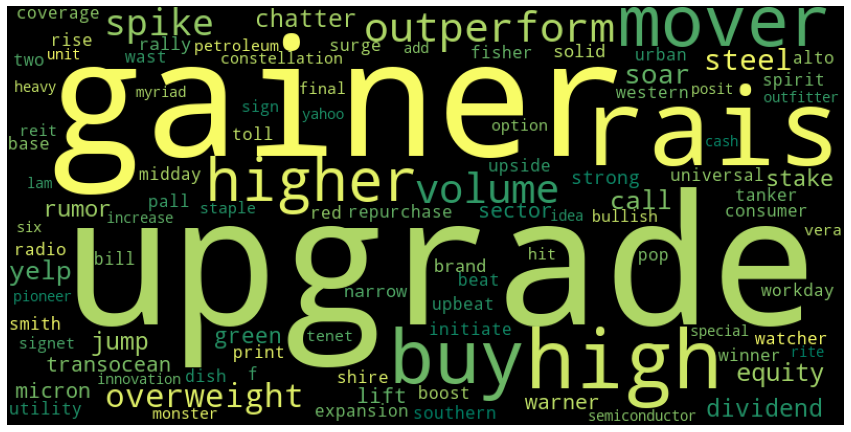
\includegraphics[scale=0.4]{pics/positive.png}
\caption{Positive words}
\end{subfigure}

\begin{subfigure}[b]{\textwidth}
\centering
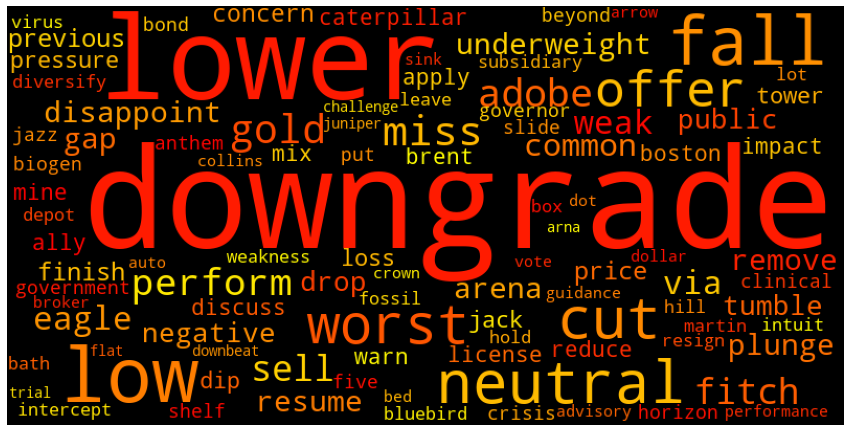
\includegraphics[scale=0.4]{pics/negative.png}
\caption{Negative words}
\end{subfigure}
\caption{Word clouds demonstrating sentiment charged words. Font size corresponds to average tone across all training samples}
\label{wordclouds}
\end{figure}

Following the construction of matrix $O$, figure \ref{wordclouds} demonstrates the list of sentiment charged words on average over all training 19 windows. At each training and validation window, the sentiment lists are generated completely from scratch, and while there is some overlap, each list can vary significantly. The font size corresponds to the average tone (calculated by $\frac{1}{2}(O_+ - O_-)$) of the words across all windows. Of the top 50 positive sentiment words, the following appeared in at least 75\% of windows, with words highlighted in \textbf{bold} appearing in all windows:
\begin{center}
      \textit{rumor, outperform, repurchase, spike, volume,} \textbf{raise, high, upgrade}
\end{center}

\noindent
The following words appear in at least 85\% of windows with respect to top 50 negative sentiment words with words highlighted in \textbf{bold} appearing in all windows:
\begin{center}
      \textit{plunge, remove, lower, public, fall,} \textbf{miss, lower, downgrade, cut, underweight}
\end{center}

Simply by inspection, each group appears reasonable, in the sense that many of the words with high values in either sentiment could be assumed. However, some words are somewhat surprising and this may offer an insight into subconsious bias that exists in writing headlines as opposed to article bodies. For example, the word \textit{volume} is, under normal circumstances, a sentiment neutral word, but according to the model generated by SESTM, is a highly positive word. Examples of headlines including this word include:
\begin{itemize}
      \item \textit{Agilent spikes to high of \$60.40 on Volume}
      \item \textit{Markets gather some momentum as volume remains light, geopolitical tension improving}
      \item \textit{Tuesday's Mid-day options for volume leaders}
\end{itemize}

Observing these headlines, it is clear that the words are being used in a positive context, and this could be due to subconscious usage of the word when constructing such headlines. However, another explanation could be overfitting. Included in the sample are headlines from `Benzinga', which is a company that offers realtime news articles, and has a significant quantity of headlines of the form \textit{Benzinga's top upgrades} (around 16,000 headlines from the entire dataset) and \textit{Benzinga's volume} (with around 2,000). This could be seen as an issue of overfitting and may skew these words' sentiment value meaning that it is not reflective of the true sentiment of the word when not used in the context of Benzinga. However, both `upgrade' and `volume' appear multiple times in the word lists for bigrams \footnote{Information on bigram computation further on} with different combinations of words, meaning that there is positive sentiment attached to these words without the context of Benzinga.

When compared to the Harvard IV and Loughran McDonald dictionaries, we find that the majority of words labelled with sentiment according to our model are not in either dictionary. The negative sentiment words have much higher overlap, with 13 of the top 50 words appearing in the LM dictionary, while only 3 appear in the H4. Conversely, only 6 words overlap LM in the positive tone, while 5 words overlap the H4 dictionary. Furthermore, many words that are included in either dictionary are determined to be sentiment neutral by the model. This is because the model is trained on a sample of headlines and the vocabulary used in headlines is vastly different to that in everyday use or 10-k filings in the case of LM. Headline vocabulary often contains much more impactful words, as it is intended to be a punchy, attention grabbing piece of text. Often, words that are typically used in headlines are rarely found outside of the context of headlines \cite{language-newspapers}. For this reason, the lexicons of the model, and that of H4 and LM differ.

\section{Daily returns}

\begin{figure}[!ht]
      \centering
\begin{tikzpicture}
\begin{axis}[scale only axis, height=8cm, width=\textwidth*.9, grid=both,
      legend pos=north west,
      date coordinates in=x, date ZERO=2019-01-01, xticklabel=\month-\year,ymin=-50,ymax=75,
      xtick={2019-01-01,2019-02-01,2019-03-01,2019-04-01,2019-05-01,2019-06-01,2019-07-01,2019-08-01,2019-09-01,2019-10-01,2019-11-01,2019-12-01,2020-01-01,2020-02-01,2020-03-01,2020-04-01,2020-05-01,2020-06-01},
      xticklabel style={
            rotate=60,
      },
       xmin=2019-01-01,
       xmax=2020-06-08]
\addplot [red, very thick, mark=none] table [header=true,x=date,y=EW-L, col sep=comma]{data/one-day-ahead.csv};
\addplot [blue, very thick, mark=none] table [header=true,x=date,y=EW-S, col sep=comma]{data/one-day-ahead.csv};
\addplot [black, very thick, mark=none] table [header=true,x=date,y=EW-LS, col sep=comma]{data/one-day-ahead.csv};
\addplot [red, very thick, dotted, mark=none] table [header=true,x=date,y=VW-L, col sep=comma]{data/one-day-ahead.csv};
\addplot [blue, very thick, dotted, mark=none] table [header=true,x=date,y=VW-S, col sep=comma]{data/one-day-ahead.csv};
\addplot [black, very thick, dotted, mark=none] table [header=true,x=date,y=VW-LS, col sep=comma]{data/one-day-ahead.csv};
\legend{L EW, S EW, LS EW, L VW, S VW, LS VW}
\end{axis}
\end{tikzpicture}
\label{graph-returns}
\caption{Cumulative log returns for each formation over the out of sample headlines}
\end{figure}

\begin{table}[!ht]
\begin{center}
\begin{tabular}{lccccccc}
      \toprule
      & Sharpe &  Average & Daily & \multicolumn{2}{c}{FF3} & \multicolumn{2}{c}{FF5} \\
      \cmidrule(lr){5-6}
      \cmidrule(lr){7-8}
      % \cmidrule(lr){9-10}
      Formation & Ratio & Return & Turnover & $\alpha$ & $R^2$ & $\alpha$ & $R^2$ \\
      \midrule
      EW L-S& 0.77 & 7.54 & 90.3\% & 5.18 & 2.83\% & 5.67 & 3.50\% \\
      EW L  & 1.05 & 12.59 & 91.83\% & 10.47 & 37.5\% & 10.37 & 38.50\% \\
      EW S  & -0.43 & -5.05 & 88.70\% & -5.29 & 21.08\% & -4.70 & 21.34\% \\
      VW L-S& 0.26 & 2.65 & 90.09\% & 0.93 & 2.32\% & 1.59 & 3.75\% \\
      VW L  & 0.35 & 4.42 & 90.38\% & 2.65 & 25.75\% & 2.72 & 27.65\% \\
      VW S  & -0.21 & -1.77 & 89.80\% & -1.72 & 24.20\% & -1.13 & 24.75\%\\
      \bottomrule
\end{tabular}
\caption{Performance of Daily News Sentiment Portfolios}
\label{portfolio-performance}
\end{center}
\end{table}


Using the headlines that were saved for out of sample testing, a portfolio is constructed for each day. On average, 353 firms have articles linked to them on a given day, and of these, almost half of these headlines contain one or more sentiment words (are not marked neutral by the model). According to the constraints ($\widehat p_i < 0.5$ for a stock to be bought, and vice versa for a stock to be sold), there are some days where less than 100 stocks form the portfolio, in which case we trade with the largest value possible. On average, the long side of the portfolio has 40 stocks, while the short side has 48, therefore the average number of stocks in the portfolio is 88.

Table \ref{portfolio-performance} describes the performance of the constructed portfolios. The two investment methods (equal and value weighted) are split up into the Long-Short combined portfolio (L-S), and the long (L) and short (S) legs are also displayed separately for comparison purposes. The daily turnover section displays the average turnover each day, which would be 100\% as the profit is liquidated at the end of each day, but some stocks are retained the following day. A turnover of 90\% (as in VW L) implies that on average 1 in 10 stocks are retained the following day. This could be due to headlines or news articles that are concerning the same events (stale news), or repeat sentiment headlines as a story unfolds over a number of days.

Unfortunately, neither of these formations are very profitable, with the only formation that is profitable being the equal weighted long strategy with a Sharpe ratio of 1.07, indicating that the profit versus risk ratio is beneficial. 

The FF3 and FF5 sections refer to Fama French 3 and 5 factor regression respectively, while the $\alpha$ concerns the intercept. The higher percentage of the average returns that the $\alpha$ value is refers to the amount of private information held in the investment. In other words, if the $\alpha$ is a very small percentage of the generated returns, then the returns that an investment has generated can be explained by regular movement in the markets, and there is no private information that is being used to generate profit.

%todo: describe what FF3 and 5 is and why anyone should care that I used it. Also describe basis points and how I calculated that. Also describe average turnover.

%todo: value weighted did better than equal weighted. This was different than when the findings from article bodies. This could be because headlines are more likely to give you information abuot big companies as this generates clicks...?

%todo: alphas are all very similar to daily turnover. Good because it means that this is something new I'm bringing to the table, not just old boring shit everyone knows already

\begin{table}[!ht]
\begin{center}
\begin{tabular}{lccccccc}
      \toprule
      & Sharpe &  Average & Daily & \multicolumn{2}{c}{FF3} & \multicolumn{2}{c}{FF5} \\
      \cmidrule(lr){5-6}
      \cmidrule(lr){7-8}
      % \cmidrule(lr){9-10}
      Formation & Ratio & Return & Turnover & $\alpha$ & $R^2$ & $\alpha$ & $R^2$ \\
      \midrule
      \multicolumn{8}{c}{Day $t-1$} \\
      EW & 18.80 & 267.01 & 90.3\% & 5.18 & 2.83\% & 5.67 & 3.50\% \\
      VW & 13.32 & 168.69 & 90.09\% & 0.93 & 2.32\% & 1.59 & 3.75\% \\
      \multicolumn{8}{c}{Day $t+0$} \\
      EW & 13.24 & 152.74 & 90.3\% & 5.18 & 2.83\% & 5.67 & 3.50\% \\
      VW & 10.70 & 101.40 & 90.09\% & 0.93 & 2.32\% & 1.59 & 3.75\% \\
      \multicolumn{8}{c}{Day $t+1$} \\
      EW & 0.77 & 7.54 & 90.3\% & 5.18 & 2.83\% & 5.67 & 3.50\% \\
      VW & 0.26 & 2.65 & 90.09\% & 0.93 & 2.32\% & 1.59 & 3.75\% \\
      \bottomrule
\end{tabular}
\caption{Performance of Daily News Sentiment Portfolios day $t-1$ to day $t+1$}
\label{portfolio-performance-day-1}
\end{center}
\end{table}

\begin{figure}[!ht]
      \centering
\begin{tikzpicture}
\begin{axis}[scale only axis, height=8cm, width=\textwidth*.9, grid=both,
      legend pos=north west,
      ymin=-15,ymax=20,
      xtick={1,2,3,4,5,6,7},
      xticklabels={Day+1, Day+2,Day+3,Day+4,Day+5,Day+6,Day+7},
      xmin=1,
      xmax=7]
\addplot [black, very thick, mark=x] table [header=true,x=day,y=avg-LS, col sep=comma]{data/speed-assimilation.csv};
\addplot [red, very thick, mark=x] table [header=true,x=day,y=avg-L, col sep=comma]{data/speed-assimilation.csv};
\addplot [blue, very thick, mark=x] table [header=true,x=day,y=avg-S, col sep=comma]{data/speed-assimilation.csv};
\legend{L-S, L, S}
\end{axis}
\end{tikzpicture}
\label{speed-assimilation}
\caption{Cumulative log returns for each formation over the out of sample headlines when headlines are considered at different delays. These formations are impossible in practice, but show the successful sentiment capture of the model}
\end{figure}


\subsection{Speed of information Assimilation}
%TODO plot graphs of day 0 to day 7 average returns to show data assimilation

\subsection{Comparison to other methods}
%TODO create table of regression on LM and H4 dictionaries to show information not captured by each

\section{What to do}

{\bf A topic-specific chapter} 
\vspace{1cm} 

\noindent
This chapter is intended to evaluate what you did.  The content is highly 
topic-specific, but for many projects will have flavours of the following:

\begin{enumerate}
\item functional  testing, including analysis and explanation of failure 
      cases,
\item behavioural testing, often including analysis of any results that 
      draw some form of conclusion wrt. the aims and objectives,
      and
\item evaluation of options and decisions within the project, and/or a
      comparison with alternatives.
\end{enumerate}

\noindent
This chapter often acts to differentiate project quality: even if the work
completed is of a high technical quality, critical yet objective evaluation 
and comparison of the outcomes is crucial.  In essence, the reader wants to
learn something, so the worst examples amount to simple statements of fact 
(e.g., ``graph X shows the result is Y''); the best examples are analytical 
and exploratory (e.g., ``graph X shows the result is Y, which means Z; this 
contradicts [1], which may be because I use a different assumption'').  As 
such, both positive {\em and} negative outcomes are valid {\em if} presented 
in a suitable manner.

% -----------------------------------------------------------------------------

\chapter{Conclusion}
\label{chap:conclusion}

\noindent
The concluding chapter of a dissertation is often underutilised because it 
is too often left too close to the deadline: it is important to allocate
enough attention to it.  Ideally, the chapter will consist of three parts:

\begin{enumerate}
\item (Re)summarise the main contributions and achievements, in essence
      summing up the content.
\item Clearly state the current project status (e.g., ``X is working, Y 
      is not'') and evaluate what has been achieved with respect to the 
      initial aims and objectives (e.g., ``I completed aim X outlined 
      previously, the evidence for this is within Chapter Y'').  There 
      is no problem including aims which were not completed, but it is 
      important to evaluate and/or justify why this is the case.
\item Outline any open problems or future plans.  Rather than treat this
      only as an exercise in what you {\em could} have done given more 
      time, try to focus on any unexplored options or interesting outcomes
      (e.g., ``my experiment for X gave counter-intuitive results, this 
      could be because Y and would form an interesting area for further 
      study'' or ``users found feature Z of my software difficult to use,
      which is obvious in hindsight but not during at design stage; to 
      resolve this, I could clearly apply the technique of Smith [7]'').
\end{enumerate}

% =============================================================================

% Finally, after the main matter, the back matter is specified.  This is
% typically populated with just the bibliography.  LaTeX deals with these
% in one of two ways, namely
%
% - inline, which roughly means the author specifies entries using the 
%   \bibitem macro and typesets them manually, or
% - using BiBTeX, which means entries are contained in a separate file
%   (which is essentially a databased) then inported; this is the 
%   approach used below, with the databased being dissertation.bib.
%
% Either way, the each entry has a key (or identifier) which can be used
% in the main matter to cite it, e.g., \cite{X}, \cite[Chapter 2}{Y}.
%
% We would recommend using BiBTeX, since it guarantees a consistent referencing style 
% and since many sites (such as dblp) provide references in BiBTeX format. 
% However, note that by default, BiBTeX will ignore capital letters in article titles 
% to ensure consistency of style. This can lead to e.g. "NP-completeness" becoming
% "np-completeness". To avoid this, make sure any capital letters you want to preserve
% are enclosed in braces in the .bib, e.g. "{NP}-completeness".

\backmatter

\bibliography{dissertation}

% -----------------------------------------------------------------------------

% The dissertation concludes with a set of (optional) appendicies; these are 
% the same as chapters in a sense, but once signaled as being appendicies via
% the associated macro, LaTeX manages them appropriatly.

\appendix

\chapter{An Example Appendix}
\label{appx:example}

Content which is not central to, but may enhance the dissertation can be 
included in one or more appendices; examples include, but are not limited
to

\begin{itemize}
\item lengthy mathematical proofs, numerical or graphical results which 
      are summarised in the main body,
\item sample or example calculations, 
      and
\item results of user studies or questionnaires.
\end{itemize}

\noindent
Note that in line with most research conferences, the marking panel is not
obliged to read such appendices. The point of including them is to serve as
an additional reference if and only if the marker needs it in order to check
something in the main text. For example, the marker might check a program listing 
in an appendix if they think the description in the main dissertation is ambiguous.

% =============================================================================

\begin{table}
      
\begin{tabular}{lcccclcccc}
\multicolumn{5}{c}{\textbf{Positive}} & \multicolumn{5}{c}{\textbf{Negative}} \\
\cmidrule(lr){1-5}
\cmidrule(lr){6-10}
Word & Sentiment & Count & LM & H4 & Word & Sentiment & Count & LM & H4 \\
\cmidrule(lr){1-5}
\cmidrule(lr){6-10}
upgrade & 0.020817 & 20 & 0 & 1 & downgrade & -0.028087 & 20 & 1 & 0 \\
raise & 0.017047 & 20 & 0 & 0 & lower & -0.018566 & 20 & 0 & 0 \\
high & 0.002975 & 20 & 0 & 0 & cut & -0.00346 & 20 & 1 & 0 \\
volume & 0.006617 & 18 & 0 & 0 & miss & -0.001796 & 20 & 1 & 0 \\
outperform & 0.003602 & 16 & 1 & 0 & underweight & -0.000875 & 20 & 0 & 0 \\
spike & 0.002856 & 16 & 0 & 0 & fall & -0.004667 & 19 & 0 & 0 \\
repurchase & 0.000383 & 16 & 0 & 0 & weak & -0.001026 & 19 & 1 & 0 \\
rumor & 0.000896 & 15 & 0 & 0 & low & -0.006097 & 18 & 0 & 0 \\
buy & 0.010115 & 14 & 0 & 0 & public & -0.000672 & 18 & 0 & 0 \\
higher & 0.006746 & 14 & 0 & 0 & plunge & -0.000851 & 17 & 0 & 0 \\
overweight & 0.001977 & 14 & 0 & 0 & remove & -0.000822 & 17 & 0 & 0 \\
green & 0.000745 & 14 & 0 & 0 & offer & -0.002654 & 16 & 0 & 0 \\
lift & 0.000786 & 13 & 0 & 0 & common & -0.00099 & 16 & 0 & 0 \\
solid & 0.000382 & 13 & 0 & 0 & disappoint & -0.000845 & 16 & 1 & 0 \\
soar & 0.001384 & 12 & 0 & 0 & negative & -0.000697 & 16 & 1 & 1 \\
strength & 0.000265 & 12 & 1 & 0 & neutral & -0.003533 & 15 & 0 & 0 \\
mention & 0.000183 & 12 & 0 & 0 & concern & -0.000515 & 15 & 1 & 0 \\
special & 0.000131 & 12 & 0 & 1 & impact & -0.000425 & 15 & 0 & 0 \\
chatter & 0.001139 & 11 & 0 & 0 & shelf & -0.00031 & 15 & 0 & 0 \\
strong & 0.000701 & 11 & 1 & 0 & weakness & -0.000259 & 15 & 1 & 0 \\
quarterly & 0.000179 & 11 & 0 & 0 & worst & -0.003078 & 14 & 1 & 1 \\
dynamics & 0.00013 & 11 & 0 & 0 & pressure & -0.000469 & 14 & 0 & 0 \\
jump & 0.000898 & 10 & 0 & 0 & resume & -0.000858 & 13 & 0 & 0 \\
upside & 0.000418 & 10 & 0 & 1 & tumble & -0.000674 & 13 & 0 & 0 \\
boost & 0.000333 & 10 & 1 & 0 & dip & -0.000481 & 13 & 0 & 0 \\
steel & 0.001527 & 9 & 0 & 0 & perform & -0.001468 & 12 & 0 & 0 \\
stake & 0.000901 & 9 & 0 & 0 & sell & -0.001288 & 12 & 0 & 0 \\
micron & 0.000816 & 9 & 0 & 0 & loss & -0.00048 & 12 & 1 & 1 \\
rally & 0.000676 & 9 & 0 & 1 & adobe & -0.001511 & 11 & 0 & 0 \\
narrow & 0.000459 & 9 & 0 & 0 & drop & -0.00069 & 11 & 0 & 0 \\
f & 0.000373 & 9 & 0 & 0 & prelim & -0.000171 & 11 & 0 & 0 \\
weigh & 9e-06 & 9 & 0 & 0 & fitch & -0.001301 & 10 & 0 & 0 \\
call & 0.001808 & 8 & 0 & 0 & beyond & -0.000341 & 10 & 0 & 0 \\
yelp & 0.001253 & 8 & 0 & 0 & challenge & -0.000199 & 10 & 1 & 0 \\
dish & 0.000812 & 8 & 0 & 0 & reduce & -0.000396 & 9 & 0 & 0 \\
dividend & 0.000809 & 8 & 0 & 0 & warn & -0.000392 & 9 & 1 & 0 \\
surge & 0.000692 & 8 & 0 & 1 & secondary & -0.000175 & 9 & 0 & 0 \\
base & 0.000419 & 8 & 0 & 0 & downside & -0.000169 & 9 & 0 & 0 \\
pop & 0.000353 & 8 & 0 & 0 & halt & -0.000165 & 9 & 1 & 0 \\
monster & 0.000286 & 8 & 0 & 0 & propose & -9.7e-05 & 9 & 0 & 0 \\
expansion & 0.000162 & 8 & 0 & 0 & community & -3.9e-05 & 9 & 0 & 0 \\
attribute & 0.000142 & 8 & 0 & 0 & four & -3.3e-05 & 9 & 0 & 0 \\
rebound & 0.000138 & 8 & 1 & 0 & gold & -0.001621 & 8 & 0 & 0 \\
unconfirmed & 0.000114 & 8 & 0 & 0 & finish & -0.000573 & 8 & 0 & 0 \\
announcement & 0.000102 & 8 & 0 & 0 & price & -0.000542 & 8 & 0 & 0 \\
declare & 6.5e-05 & 8 & 0 & 0 & mix & -0.000368 & 8 & 0 & 0 \\
test & 3.2e-05 & 8 & 0 & 0 & license & -0.00036 & 8 & 0 & 0 \\
improve & 3e-05 & 8 & 1 & 0 & slide & -0.000283 & 8 & 0 & 0 \\
urban & 0.000528 & 7 & 0 & 0 & leave & -0.00023 & 8 & 0 & 0 \\
beat & 0.000459 & 7 & 0 & 0 & bed & -0.000217 & 8 & 0 & 0 \\
\bottomrule
\end{tabular}
\caption{Top sentiment words for each polarity, along with appearance in either Loughran McDonald dictionary (LM) or Harvard IV psychological dictionary (H4). Note sentiment in this case refers to average \textit{tone} over all 20 training windows. Words are first sorted via count of training windows appeared in, and then by sentiment}
\end{table}
\end{document}
